\section{A Survey on 5G Network Technologies from a Social Perspective}
\textcolor{black}{The rapid advancement in communication technology innovations results in proliferation of heterogeneous smart devices in the network. The inter-communication of these devices is usually related to their social behavior and relationships. Furthermore, the upcoming 5G network promises to bind all the network technologies like Internet of Vehicles (IoV), Internet of Things (IoT), Mobile Cloud Computing (MCC), Smart Grids (SG), Big Data, and Device-to-Device (D2D) communications in a common network. To achieve this unified goal, one promising possibility is to exploit social properties of various smart devices used by these technologies. Exploitation of social aspect can dispense optimized networking while avoiding problems such as network congestion, resource allocations, and the like. It also leads to convergence of upcoming 5G network technologies and human society, giving rise to a new paradigm known as “socio-5G network technologies”. The state-of-the-art research on socio-5G network technologies is reviewed with the focus on six important technologies that 5G promises to support in one integrated network: IoV, IoT, MCC, SG, Big Data, and D2D communications. We also discuss the open issues related to combining social aspects with above-mentioned technologies.}
% \section{Results}
% Lorem ipsum dolor sit amet, consectetur adipiscing elit. Duis ut ipsum nec orci interdum sollicitudin ut eu nunc. Pellentesque 

% % \textcolor{red}{When placing tables (\autoref{tab:econ}) within the body of the text, the citation is placed above the table.} 

% \begin{figure}
%     \centering
%     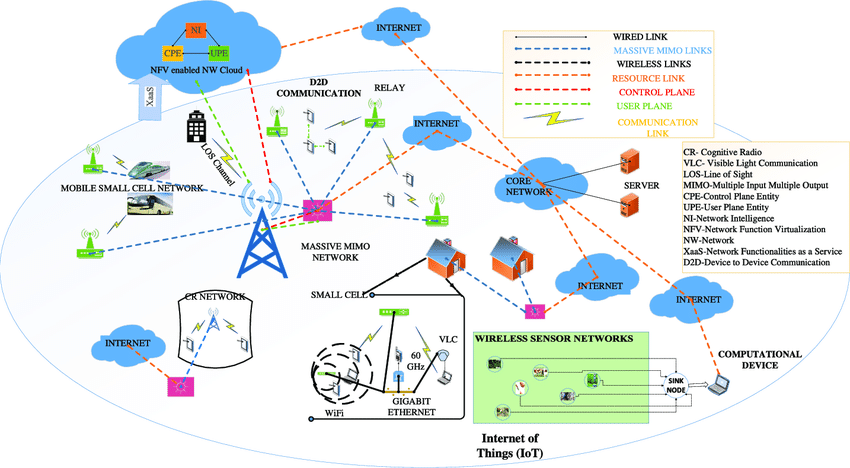
\includegraphics[width=17cm]{Images/result.png}
%     \caption{Result}
%     \label{fig:my_label}
% \end{figure}

% \begin{table}[!ht]
%   \centering
%   {\small {\it \caption{The economic argument \label{tab:econ} \hcite{econ}}}}
%   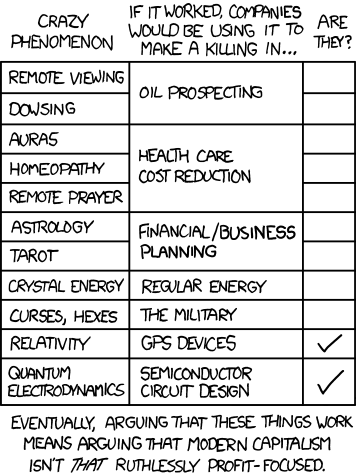
\includegraphics [scale=0.5]{Images/the_economic_argument.png} \\
% \end{table}

% \vfill

\newpage 

\section{Discussion}
\textbf{Sukhdeep Singh}Sukhdeep Singh completed his bachelor’s and master’s degree in technology from GyanVihar University, Jaipur, India. Currently, he is a PhD research scholar in the ECE Department of the College of Information and Communication Engineering, Sungkyunkwan University, South Korea. His research interests are mobile video streaming in social networks, cloud computing, and green networking. He has presented at five international conferences and has two journal publications.\item\textbf{Navrati Saxena}is an associate professor in the Electrical Engineering Department, Sungkyunkwan University, South Korea. She worked as an \item\textbf{Abhishek Roy}is currently working in the System Design Lab of Networks Systems Division, Samsung Electronics in South Korea. He received his PhD degree in 2010 from Sungkyunkwan University in the College of Information and Communication Engineering, MS degree in 2002 from the University of Texas at Arlington, USA, and BE degree in 2000 from Jadavpur University, India. His research interests include different mobility and resource management aspects of 4G wireless systems. He served as the lead guest editor of Springer EURASIP Journal of Wireless Communications and Networking and in the technical program committee of many international conferences. He has co-authored one book (published by Taylor and Francis, USA) and published more than 20 international journals and presented at more than 20 international conferences.

% \textcolor{red}{When placing figures (illustrations, pictures, graphs, diagrams, charts, maps etc.) within the body of the text, the citation is placed below the figure (\autoref{fig:moun})}

% \begin{figure}[!h]
%   \centering
%   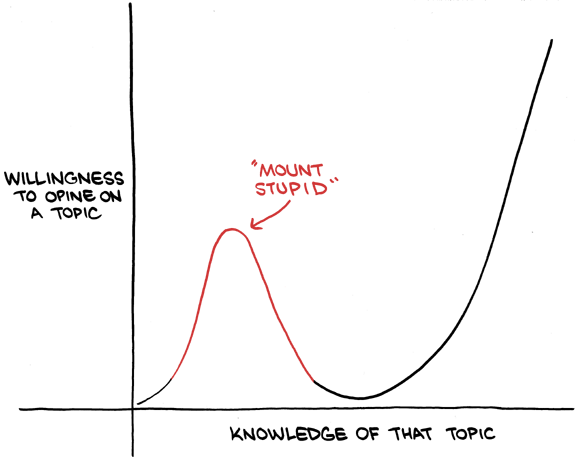
\includegraphics [scale=0.5]{Images/dunning_kruger.png} \\
%   {\small {\it \caption{Dunning–Kruger effect \label{fig:moun} \hcite{mount}}}}
% \end{figure}